\documentclass{article}
\usepackage[utf8]{inputenc}
\usepackage[spanish]{babel}
\usepackage{graphicx, graphics, float, fancyhdr, titling}
\usepackage{listings, subcaption}
\usepackage[a4paper, total={6in, 9.5in}]{geometry}
\usepackage{hyperref}
\renewcommand{\footrulewidth}{0.4pt}
\title{

\includegraphics[width=1.75in]{imagenes/UGR-Logo.png} \\
\vspace*{1in}
\textbf{Práctica 1, Sesión 5} \\
Seguridad en Sistemas Operativos \\
\vspace*{0.5in}}
\author{Andrés Merlo Trujillo \\
\vspace*{0.5in} \\
E.T.S. de Ingenierías Informática y de Telecomunicación \\
\textbf{Universidad de Granada}} \date{\today}
%\date{}
\hypersetup{
    colorlinks=true,
    linkcolor=black,
}

\renewcommand\maketitlehooka{\null\mbox{}\vfill}
\renewcommand\maketitlehookd{\vfill\null}

\begin{document}
\begin{titlingpage}
    \maketitle
\end{titlingpage}

\tableofcontents

\newpage

\pagestyle{fancy}
\fancyhead[L]{Andrés Merlo Trujillo}
\fancyhead[R]{Seguridad en Sistemas Operativos}
%\addcontentsline{toc}{section}{Ejercicio 1}
%\section{Ejercicio 1}
%\begin{figure}[H]
%    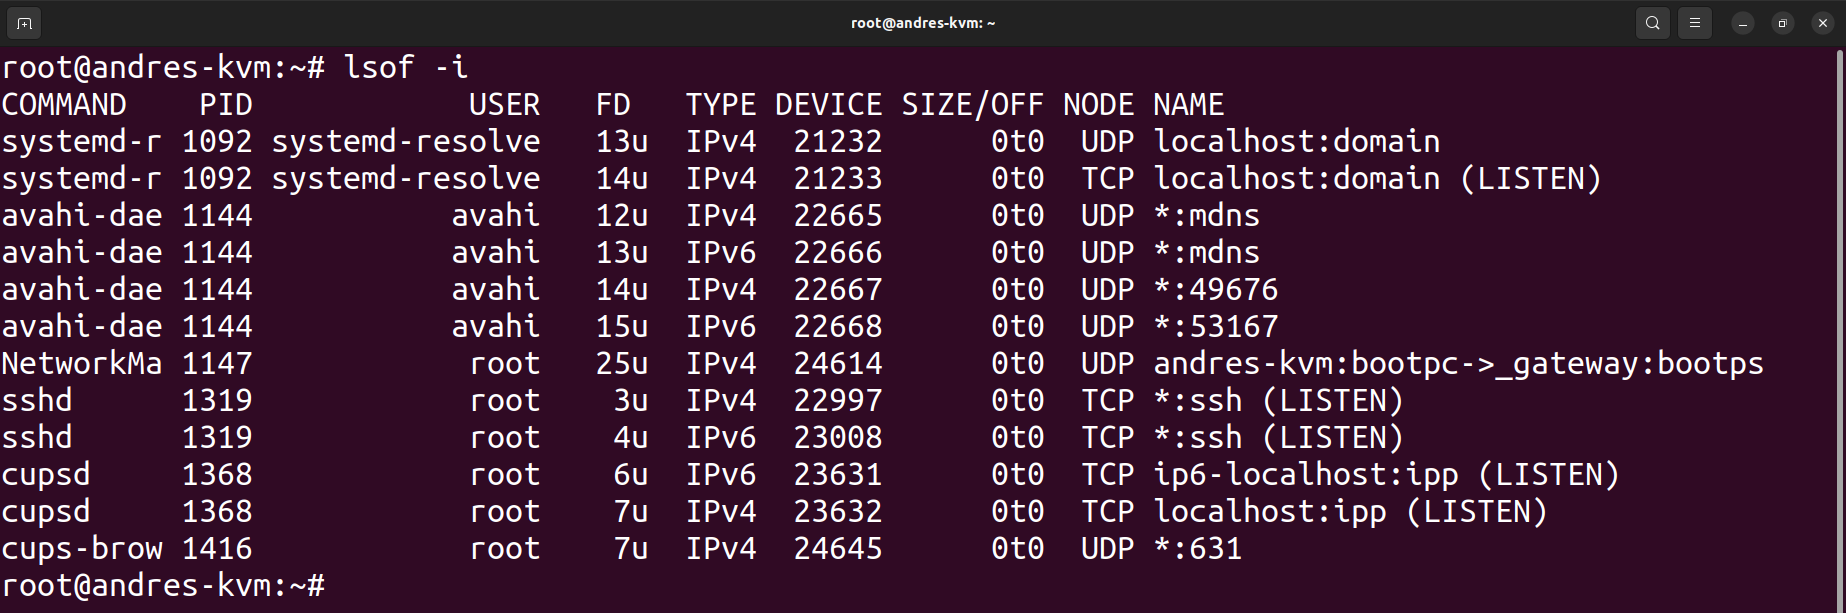
\includegraphics[width=\textwidth]{imagenes/lsofi.png}
%\end{figure}

%\addcontentsline{toc}{section}{Ejercicio 1}
%\section{Ejercicio 1}
\section{Ejercicio 1}

\textbf{Enunciado: }``Utilizar \texttt{cryptsetup} para crear una partición encriptada en un pendrive. Escribir un archivo en él. Desmontarlo y extraerlo. ¿Qué ocurre cuando volvemos a conectarlo?''

\bigskip

Lo primero que hay que hacer es encriptar el pendrive, esto se puede hacer ejecutando la orden \verb|cryptsetup luksFormat /dev/device| (en mi caso es \verb|/dev/sda|, ya que estoy en una máquina virtual con un pendrive pasado por passthrough). Es importante recordar que el dispositivo no debe estar montado en ningún sitio, si lo estuviera con la orden \verb|umount punto_montaje| se desmonta.

\begin{figure}[H]
    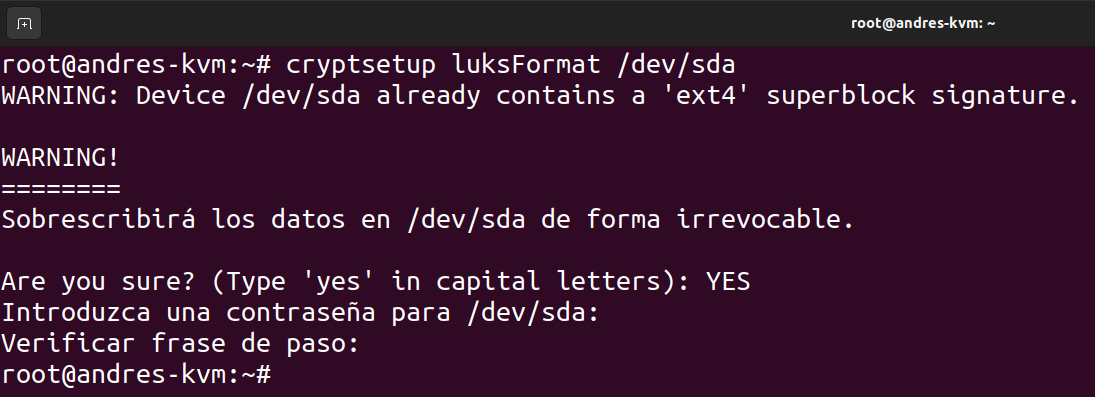
\includegraphics[width=\textwidth]{imagenes/Captura desde 2022-10-30 10-51-54.png}
    \caption{Formateo de la partición para ser un contenedor LUKS.}
\end{figure}

\bigskip

Como se puede ver, pide una contraseña de cifrado para encriptar el dispositivo. Una vez encriptado, es necesario abrirlo, se puede hacer con la orden \verb|cryptsetup open /dev/device nombre|, donde nombre indica el nombre que se le pondrá al ser abierto (para acceder a él es necesario buscarlo en la ruta \verb|/dev/mapper/nombre|):

\begin{figure}[H]
    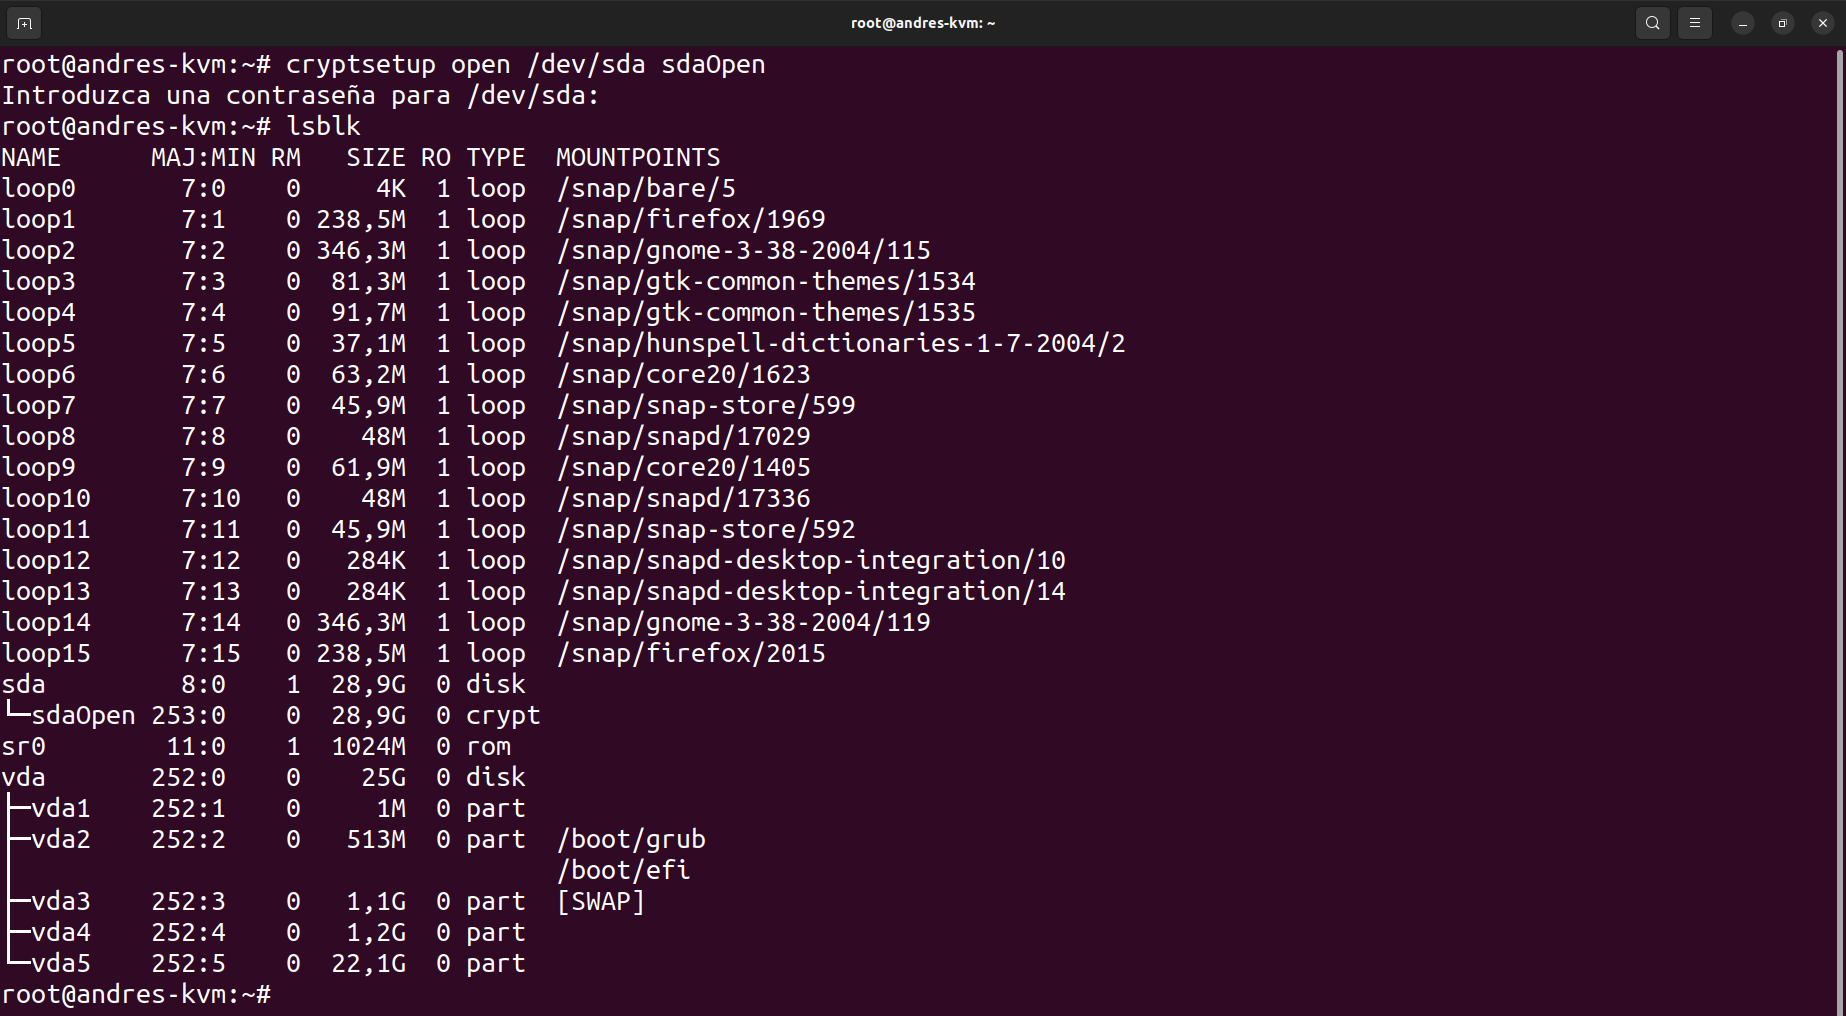
\includegraphics[width=\textwidth]{imagenes/Captura desde 2022-10-30 10-54-01.png}
    \caption{Contenedor LUKS desencriptado.}
\end{figure}

\newpage

Una vez abierto, es necesario crear un sistema de archivos para que se pueda trabajar con él. Esto se puede hacer con la orden \verb|mkfs.ext4 /dev/mapper/device|:

\begin{figure}[H]
    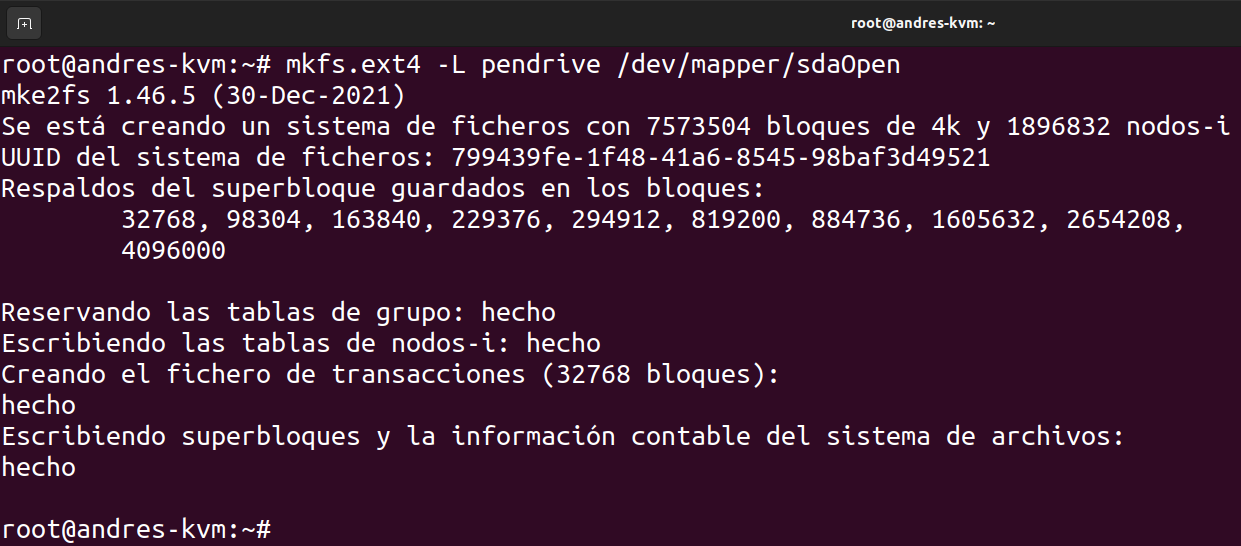
\includegraphics[width=\textwidth]{imagenes/Captura desde 2022-10-30 10-57-11.png}
    \caption{Creación del sistema de archivos dentro del contenedor LUKS.}
\end{figure}

\bigskip

Y ahora, se puede usar la orden \verb|mount /dev/mapper/device punto_montaje| como cualquier otro dispositivo.

\begin{figure}[H]
    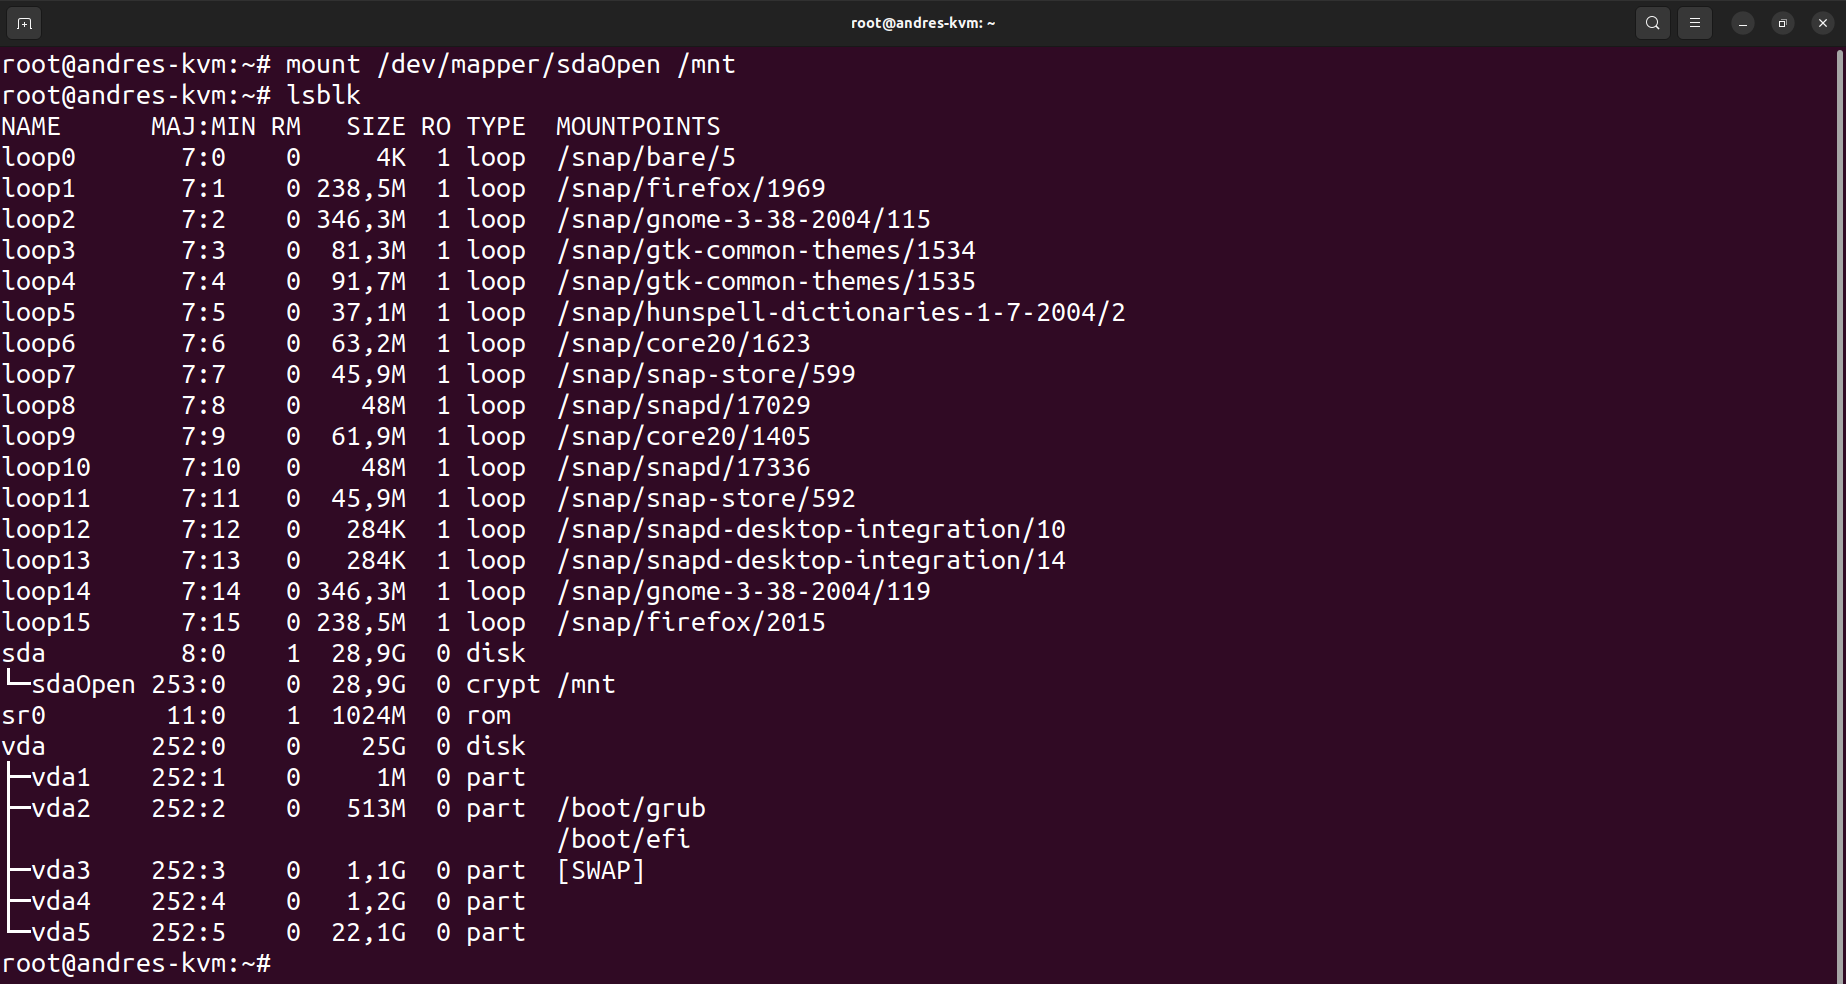
\includegraphics[width=\textwidth]{imagenes/Captura desde 2022-10-30 10-58-23.png}
    \caption{Montaje del sistema de archivos desencriptado.}
\end{figure}

\newpage

A continuación, voy a crear el siguiente archivo con algo de texto en su interior:

\begin{figure}[H]
    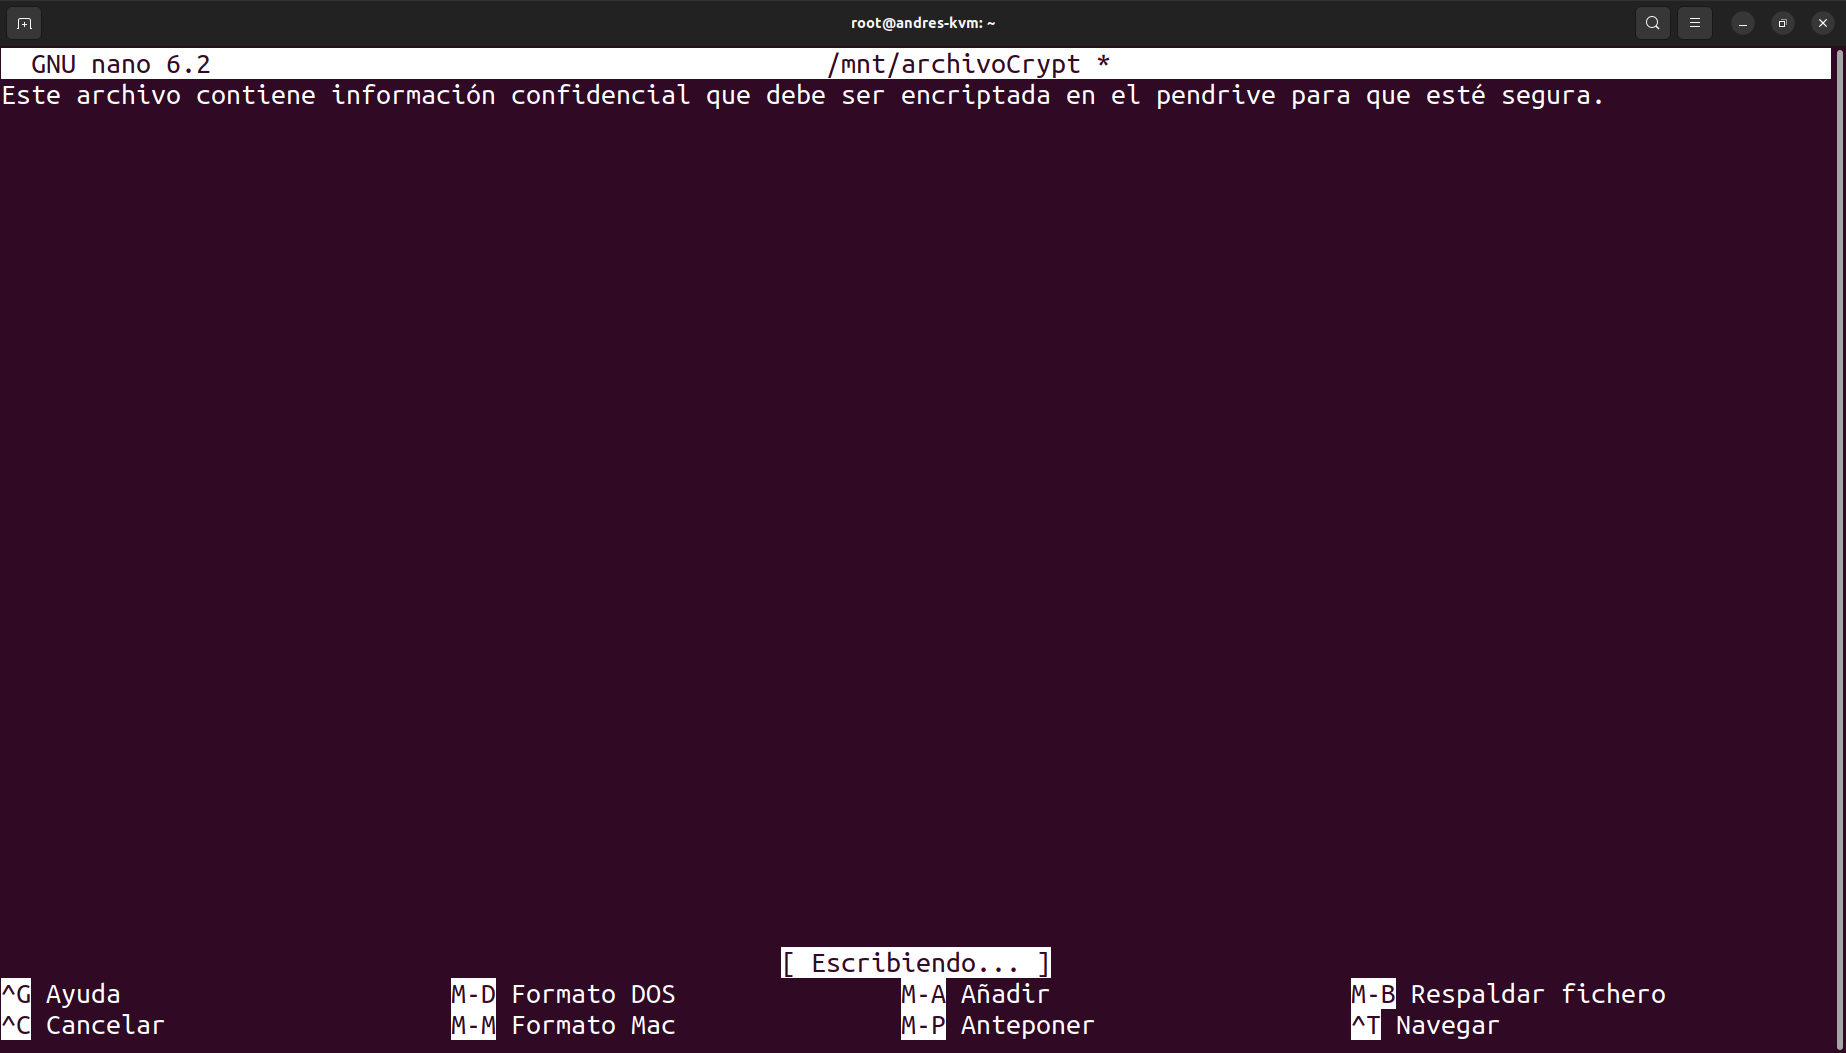
\includegraphics[width=\textwidth]{imagenes/Captura desde 2022-10-30 10-59-27.png}
    \caption{Archivo a encriptar.}
\end{figure}

\bigskip

Seguidamente, es necesario desmontar el sistema de archivos primero y luego cerrar la partición cifrada. Esto primero se puede hacer con la orden \verb|umount punto_montaje|.

\begin{figure}[H]
    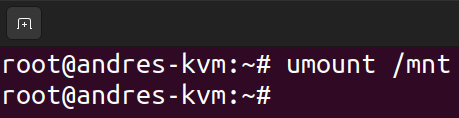
\includegraphics[width=\textwidth]{imagenes/Captura desde 2022-10-30 11-00-34.png}
    \caption{Desmontaje de la partición desencriptada.}
\end{figure}

\bigskip

Lo siguiente es cerrar la partición encriptada.

Esto se realiza ejecutando la orden \verb|cryptsetup close /dev/mapper/device|


\begin{figure}[H]
    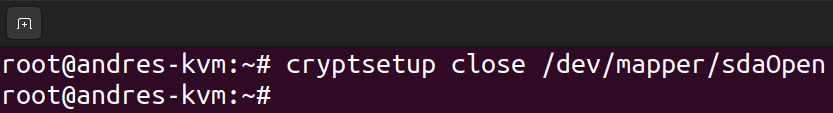
\includegraphics[width=\textwidth]{imagenes/Captura desde 2022-10-30 11-02-02.png}
    \caption{Cierre del contenedor LUKS.}
\end{figure}

\bigskip

El último paso que se explica a continuación paso es opcional, ya que es imposible que se pueda escribir nada en el dispositivo estando desmontado, pero se puede ejecutar la orden \verb|eject /dev/sda| o hacerlo desde el entorno de escritorio para expulsar el dispositivo.

\begin{figure}[H]
    \centering
    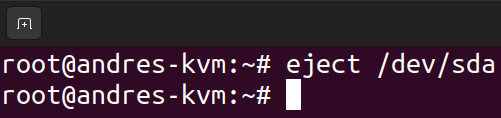
\includegraphics[width=0.6\textwidth]{imagenes/Captura desde 2022-10-30 11-03-16.png}
    \caption{Extracción del pendrive.}
\end{figure}

Ahora al volverlo a conectar, GNOME pide la contraseña para desencriptar.

\begin{figure}[H]
    \centering
    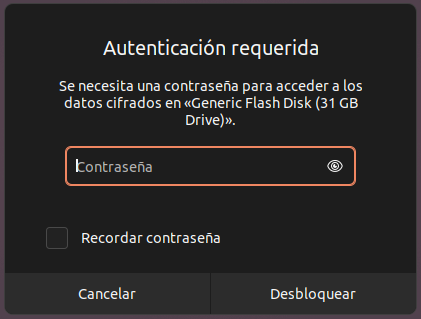
\includegraphics[width=0.5\textwidth]{imagenes/Captura desde 2022-10-30 11-04-17.png}
    \caption{Pantalla para introducir la contraseña de cifrado.}
\end{figure}

\bigskip

Una vez desencriptado, GNOME lo monta de manera automática, haciendo accesible el contenido del pendrive.

\begin{figure}[H]
    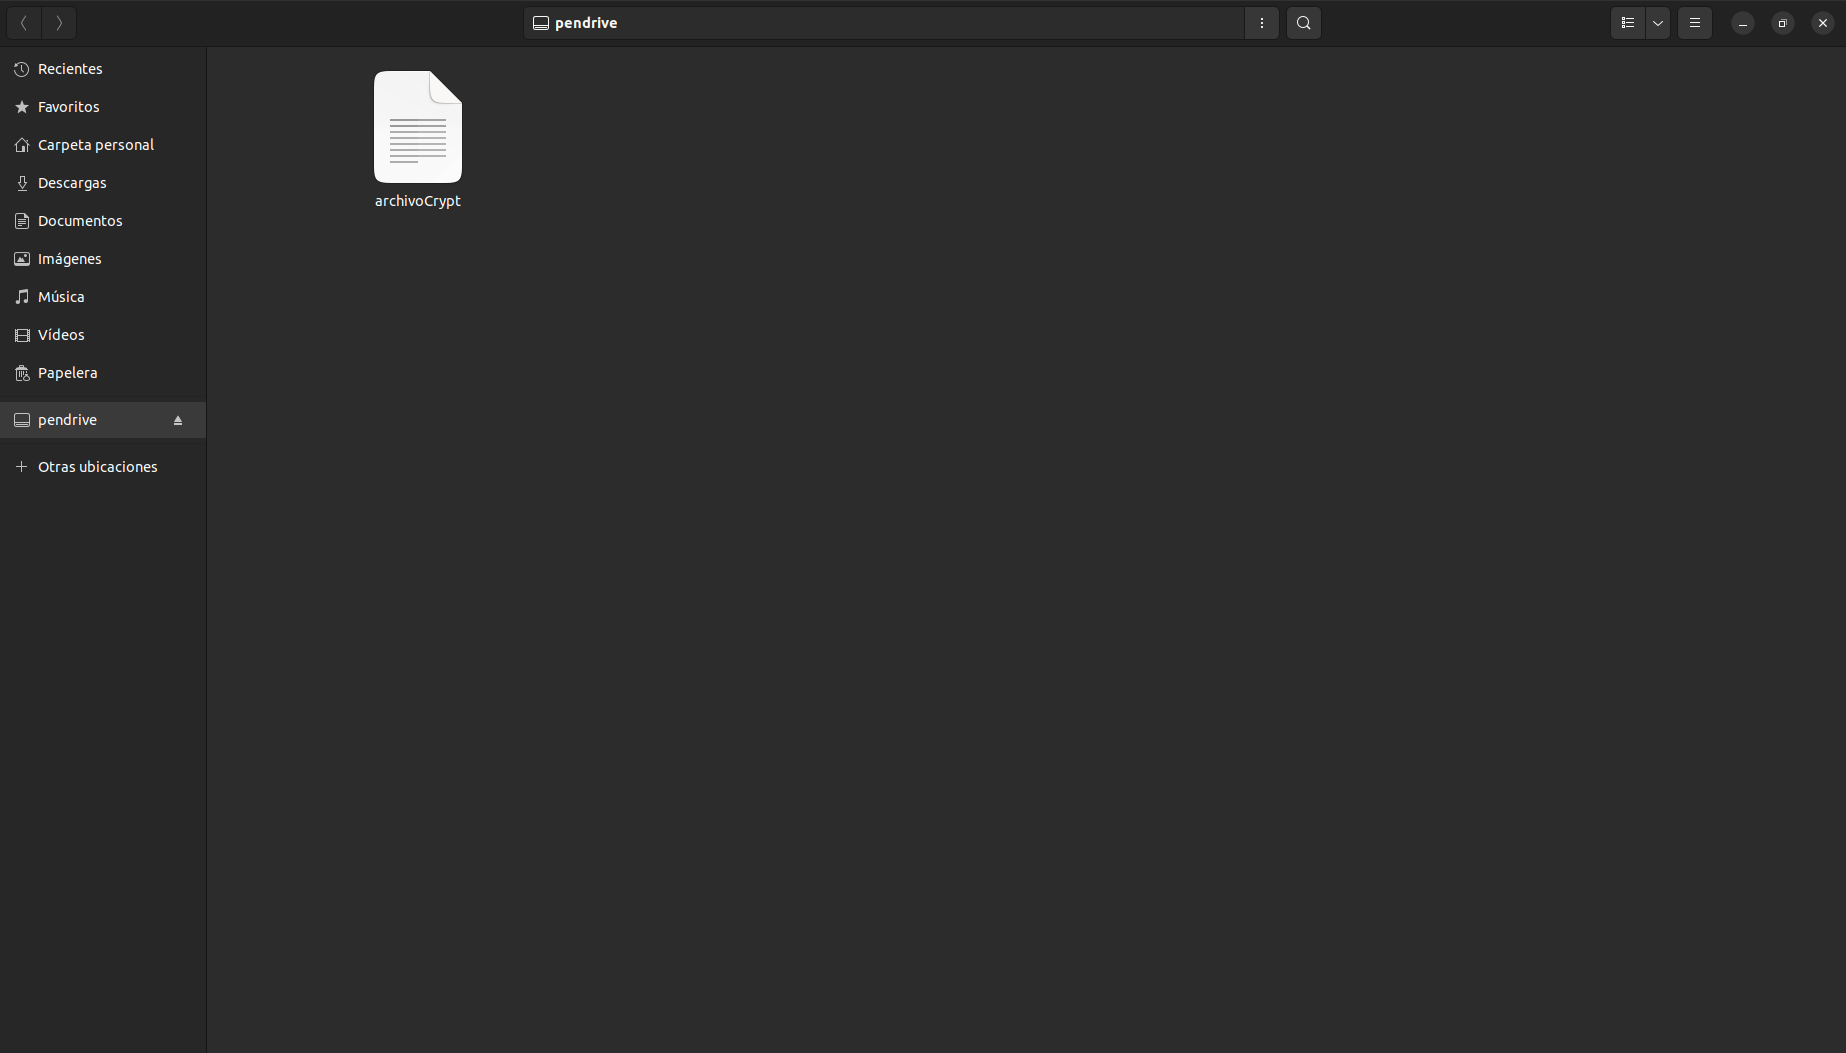
\includegraphics[width=\textwidth]{imagenes/Captura desde 2022-10-30 11-05-16.png}
    \caption{Contenido del pendrive cifrado.}
\end{figure}

\begin{figure}[H]
    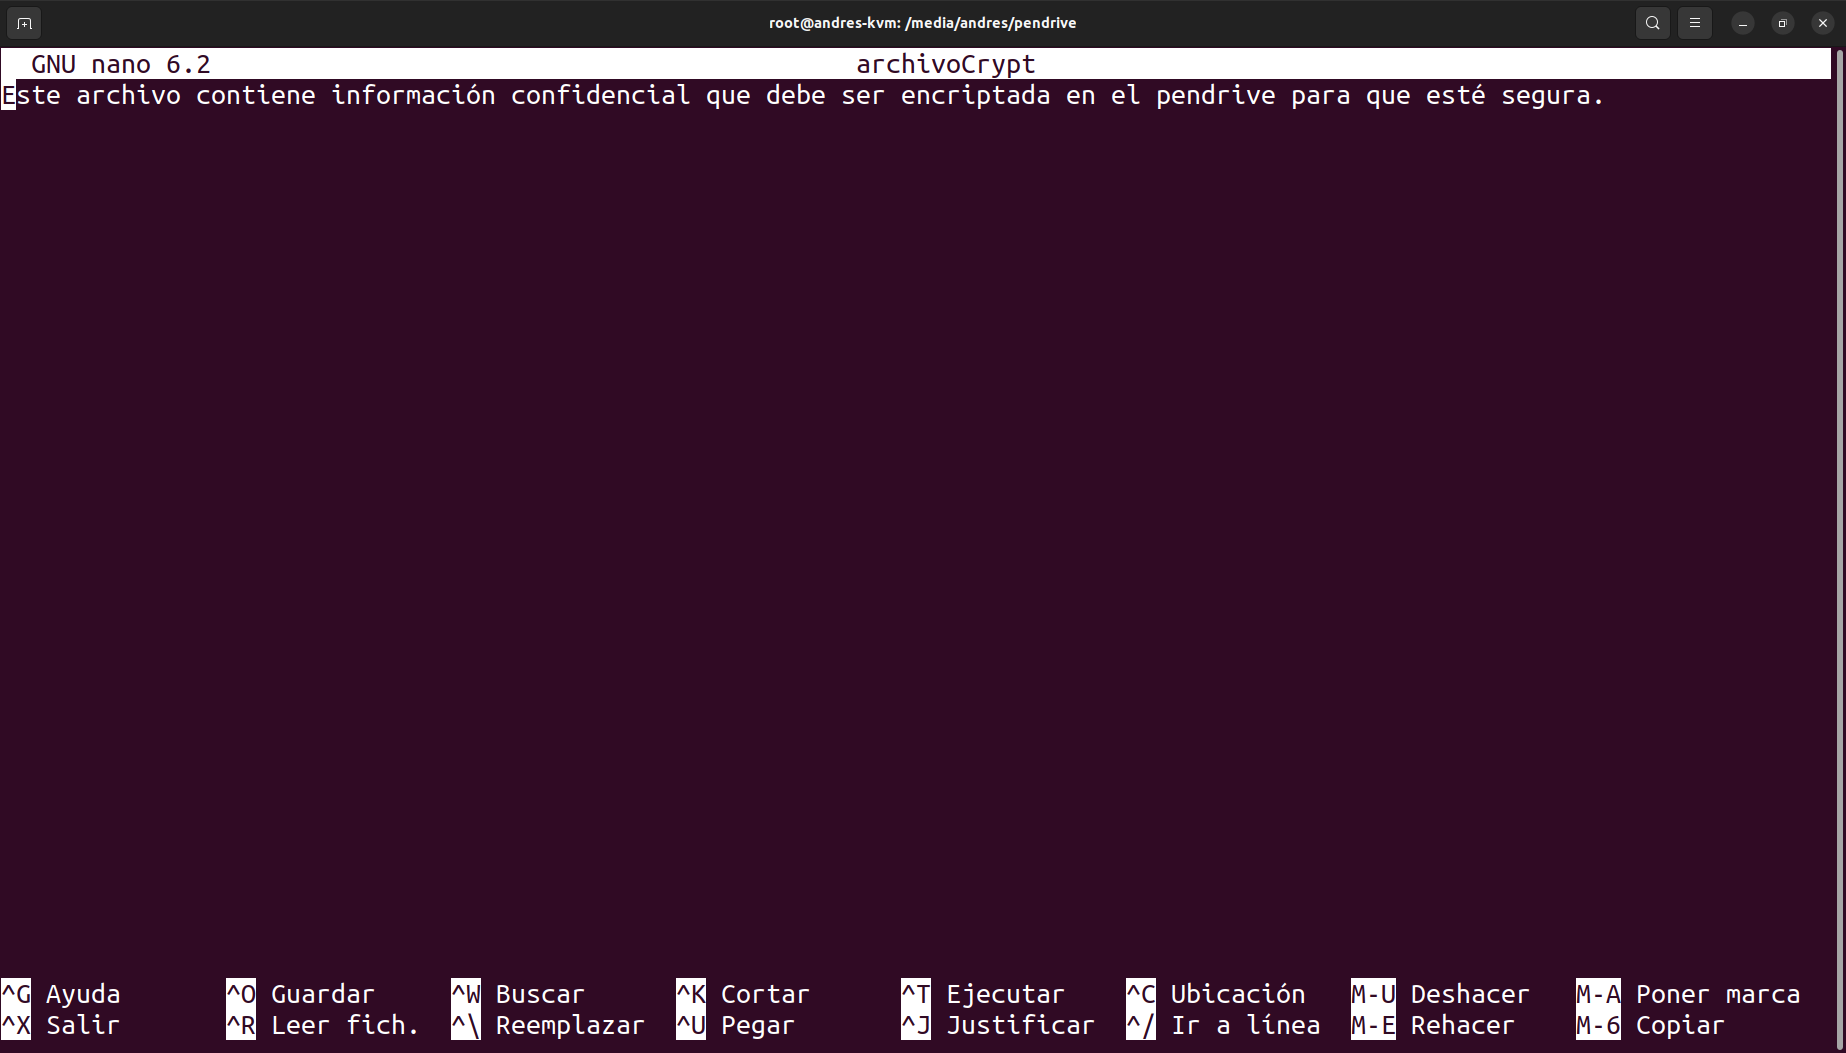
\includegraphics[width=\textwidth]{imagenes/Captura desde 2022-10-30 11-05-44.png}
    \caption{Contenido del archivo cifrado del pendrive.}
\end{figure}

\bigskip

Todo esto se podría haber hecho de manera manual mediante terminal realizando los comandos anteriormente mencionados en este orden:

\begin{enumerate}
    \item \verb|cryptsetup open /dev/sda sdaOpen|
    \item \verb|mount /dev/mapper/sdaOpen /mnt|
\end{enumerate}

Sin embargo, para el usuario promedio es mejor realizarlo de manera gráfica, como lo que ofrecen entornos de escritorio como GNOME o KDE.

\newpage

\section{Ejercicio 2}

\textbf{Enunciado: }``Utilizar la herramienta \textit{Steghide} para ocultar un mensaje dentro de una imagen, tal como acabamos de ver. Comparar los archivos portador antes y después de usar la técnica para ver las diferencias.''

\bigskip

Para instalar ``Steghide'' en Ubuntu es necesario usar la orden \verb|sudo apt install steghide|

\bigskip

Voy a usar la siguiente imagen para ocultar un mensaje con la herramienta:

%imagen
\begin{figure}[H]
    \centering
    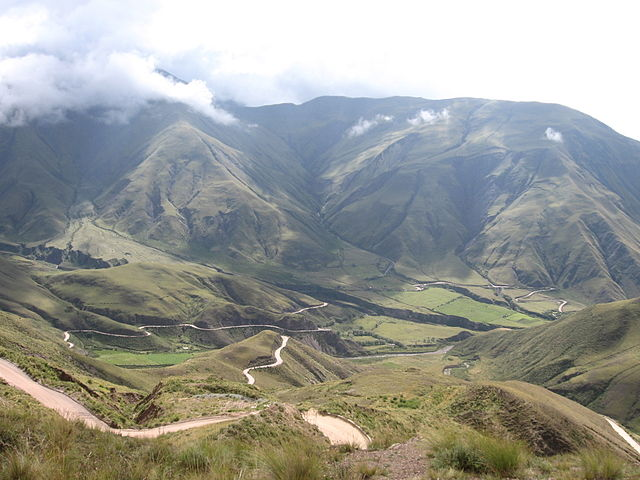
\includegraphics[width=0.7\textwidth]{imagenes/imagen.jpg}
    \caption{Imagen a la que se le va a realizar estenografía.}
\end{figure}

Y voy a ocultar el siguiente mensaje:

\begin{figure}[H]
    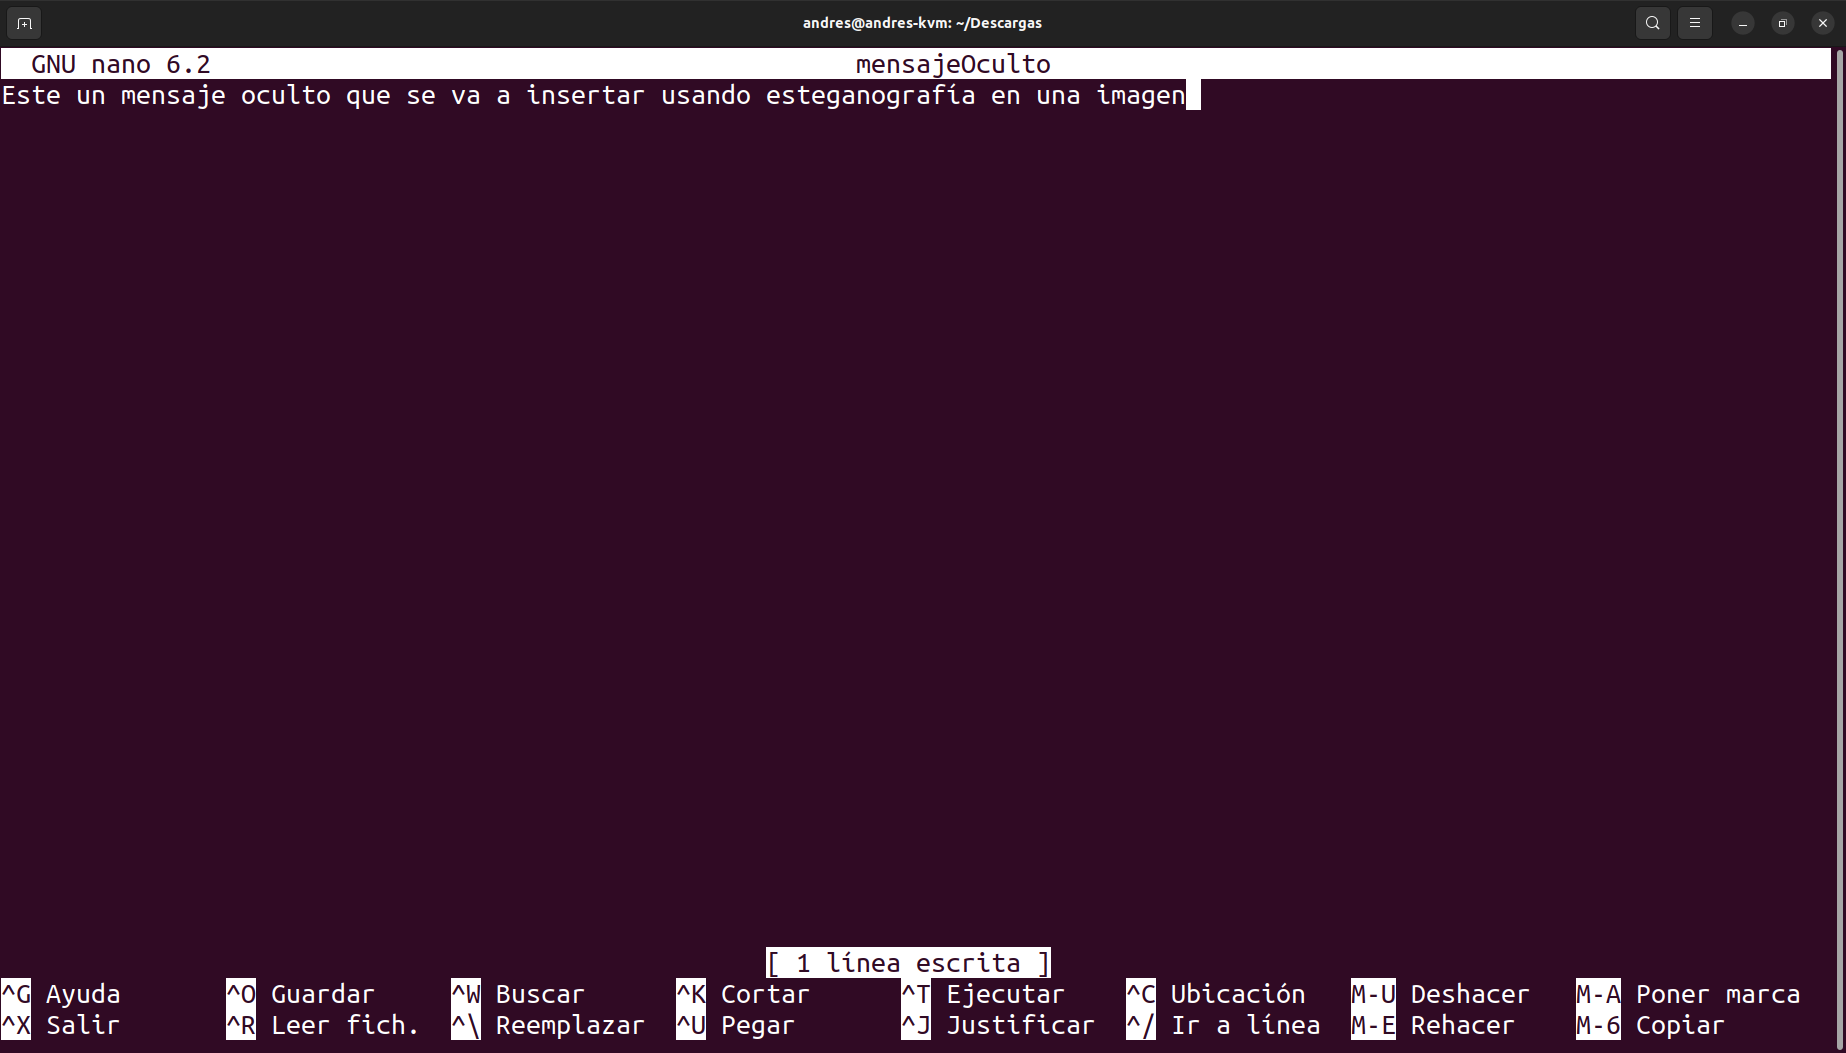
\includegraphics[width=\textwidth]{imagenes/Captura desde 2022-10-30 11-27-46.png}
    \caption{Mensaje que se va a insertar en la imagen.}
\end{figure}

\bigskip

Finalmente, para ocultar el mensaje en la imagen se usa la orden:

\verb|steghide embed -cf imagen -ef texto|

\begin{figure}[H]
    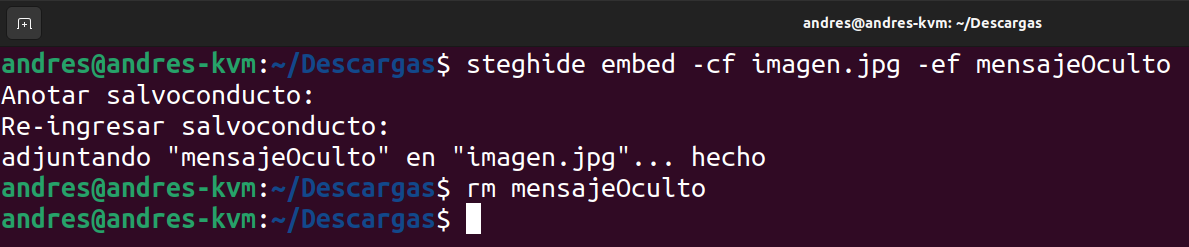
\includegraphics[width=\textwidth]{imagenes/Captura desde 2022-10-30 11-30-08.png}
    \caption{Inserción del mensaje en la imagen.}
\end{figure}

\bigskip

Como se puede observar, pide un salvoconducto, que es una contraseña que hay que introducir para que se pueda extraer el contenido de la imagen.

\bigskip

Ahora, al comparar las dos imágenes, a simple vista no se puede observar ninguna diferencia aparente.

%imagen imagenMod
\begin{figure}[H]
    \centering
    \begin{subfigure}[H]{0.49\textwidth}
        \centering
        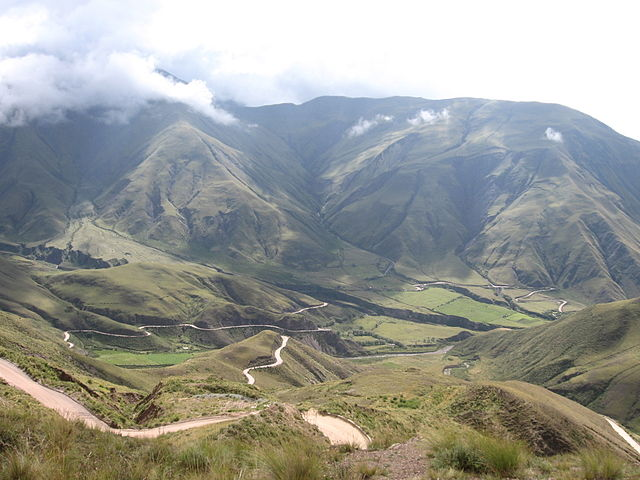
\includegraphics[width=\textwidth]{imagenes/imagen.jpg}
        \caption{Imagen original (sin modificar).}
    \end{subfigure}
    \hfill
    \begin{subfigure}[H]{0.49\textwidth}
        \centering
        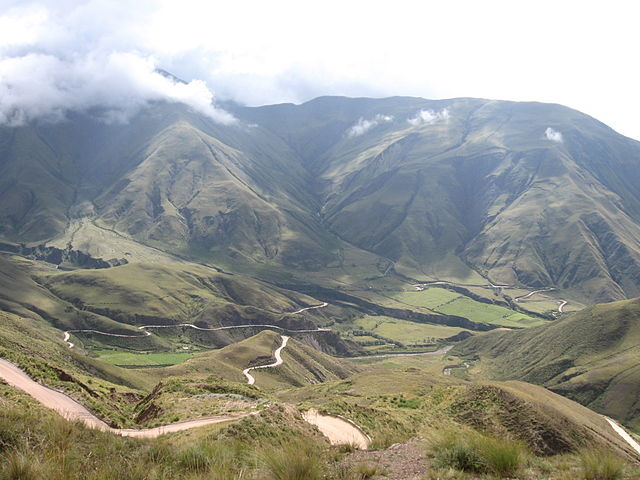
\includegraphics[width=\textwidth]{imagenes/imagenMod.jpg}
        \caption{Imagen con archivo oculto.}
    \end{subfigure}    
    \caption{Comparativa de imagen original con la que tiene el archivo oculto.}
\end{figure}

A continuación, al comparar sus hashes podemos ver que son completamente distintos.

\begin{figure}[H]
    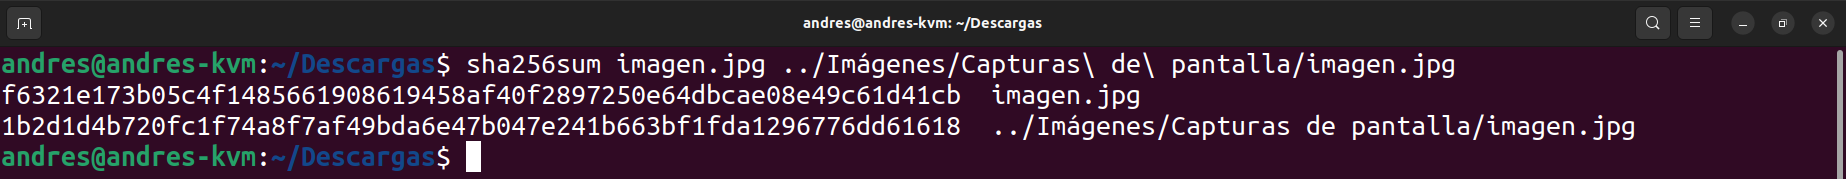
\includegraphics[width=\textwidth]{imagenes/Captura desde 2022-10-30 11-38-52.png}
    \caption{Diferencias hash de las dos imágenes.}
\end{figure}

\newpage

Ahora bien, existe la orden \verb|compare| que permite comparar dos imágenes y obtener el resultado en otra imagen mostrando como píxeles rojos aquellos que han sido modificados de la imagen original. Usando la orden \verb|compare image1 image2 -compose src diff.png| se puede obtener la siguiente imagen:

\begin{figure}[H]
    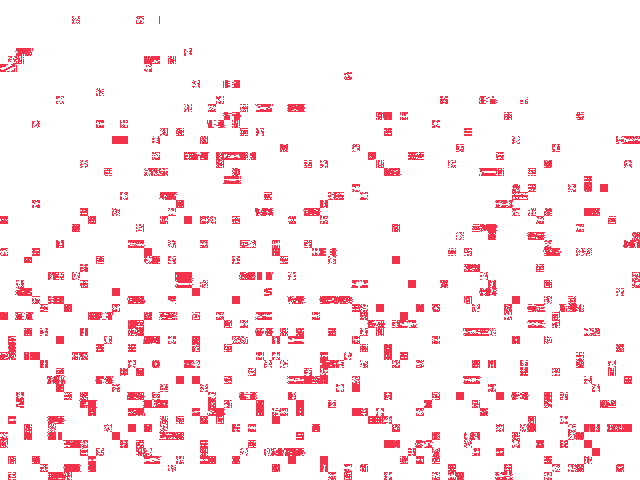
\includegraphics[width=\textwidth]{imagenes/diff.png}
    \caption{Diferencias a nivel de píxeles de ambas imágenes.}
\end{figure}

\bigskip

Como se puede ver, han sido modificados muchos píxeles de la imagen original.

\bigskip

Finalmente, con la orden \verb|steghide extract -sf imagen.jpg| se puede obtener el archivo oculto en la imagen.

\begin{figure}[H]
    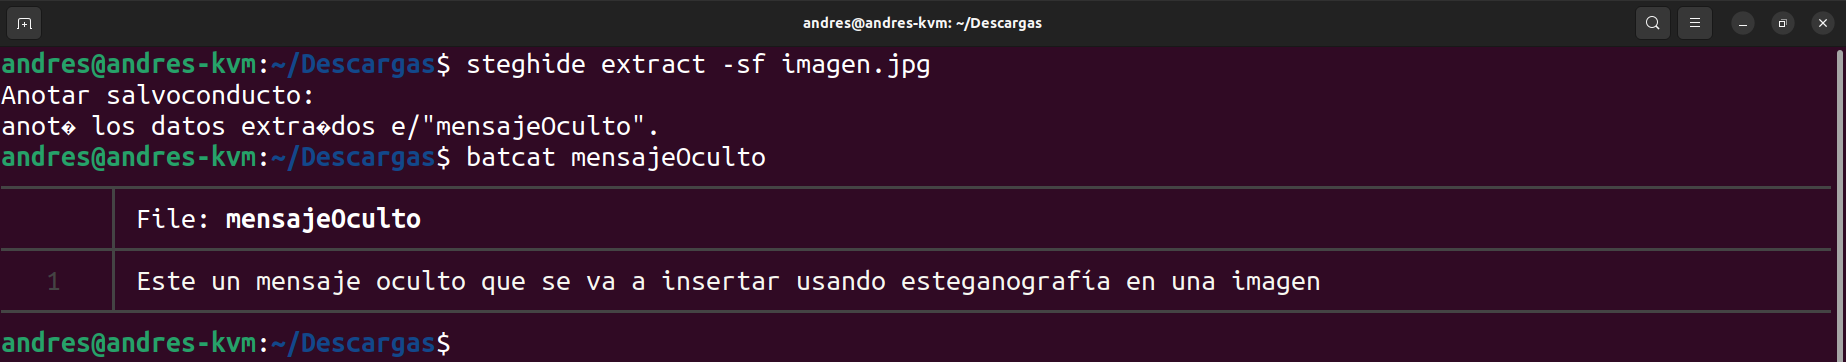
\includegraphics[width=\textwidth]{imagenes/Captura desde 2022-10-30 11-44-23.png}
    \caption{Obtención del mensaje oculto.}
\end{figure}

\bigskip

Como se puede observar, pide la contraseña que se pedía al insertar el archivo en la imagen.

\newpage

\section{Ejercicio 3}

\textbf{Enunciado: }``Utilizar VSL para analizar la imagen esteganográfica generada en el ejercicio anterior para detectar información oculta.''

\bigskip

Por desgracia, no he sido capaz de poder ejecutar el programa VSL de ninguna forma. He probado con Ubuntu 22.04.1 LTS y Arch Linux actualizado a día 30 de octubre de 2022 y con varias versiones de JDK (8, 11, 18 y 19). Con ninguna de estas combinaciones ha funcionado. 

\bigskip

Lo máximo que he conseguido ha sido que arrancase el programa, modelar el input, el decodificador y el output y elegir la imagen con el archivo oculto. Sin embargo, al darle a ejecutar experimento se produce una excepción de Java que me impide continuar.

\bigskip

Cabe destacar que he probado con Windows 11 también y se produce exactamente el mismo error.

\begin{figure}[H]
    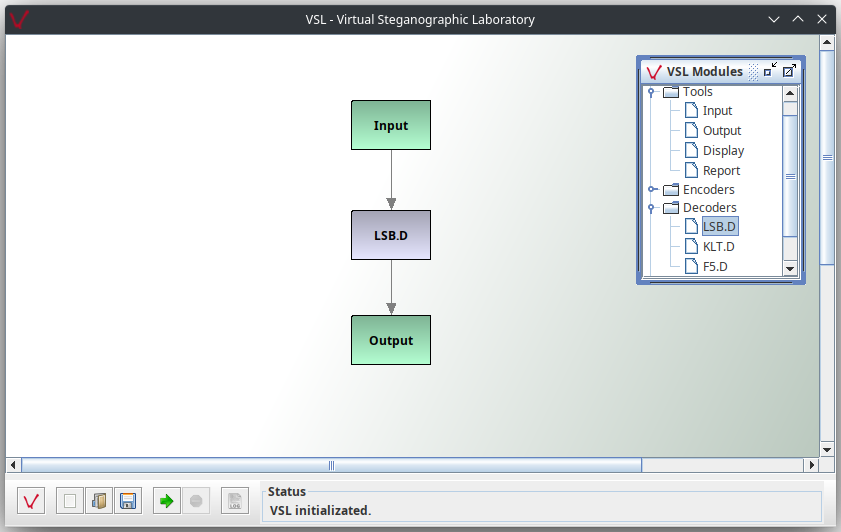
\includegraphics[width=\textwidth]{imagenes/Screenshot_20221030_152701.png}
    \caption{Estructura que debería haber tenido el decodificador.}
\end{figure}

\begin{figure}[H]
    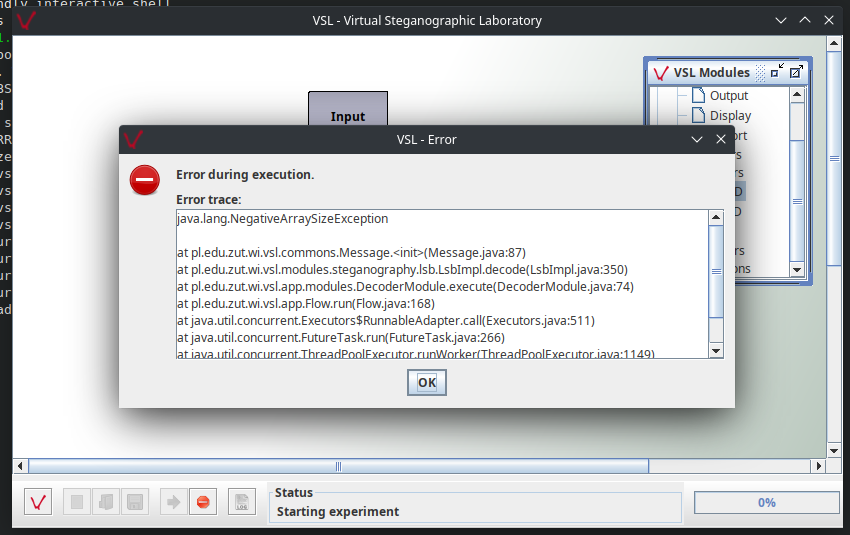
\includegraphics[width=\textwidth]{imagenes/Screenshot_20221030_145831.png}
    \caption{Error que aparece al intentar ejecutar el programa.}
\end{figure}

%Nota: El programa no he sido capaz de ejecutarlo usando Ubuntu 22.04.1 LTS. He probado con varias versiones de JDK, pero siempre saltaba con alguna excepción de Java y la ventana no se conseguia abrir. Finalemnte he optado por pasar las imagenes a otra maquina virtual que utiliza Arch Linux y en la que si puedo ejecutar el programa con OpenJDK 8.
%
%
%Primero hay que descargar el programa usando el siguiente enlace: \url{http://vsl.sourceforge.net/}.
%
%Una vez hecho esto, se descomprime y usando el comando \verb|java -jar programa.jar| se ejecuta (es necesario tener openjdk instalado).
%
%%FOTO D LA PANTALLA INICIAL
%
%Ahora hace falta conectar como aparece en el video un ``Input'', con el decodificador ``LSB.D'' y finalmente el Output. Luego, haciendo click derecho, se le da a ``Connect'' y se conectan.
%
%%foto del esquema
%
%Lo siguiente que hay que hacer, es añadirle la imagen en el input modificada, para ello, se le da click derecho y se elige la opcion ``select input''.
%
\end{document}

%\begin{figure}[H]
%    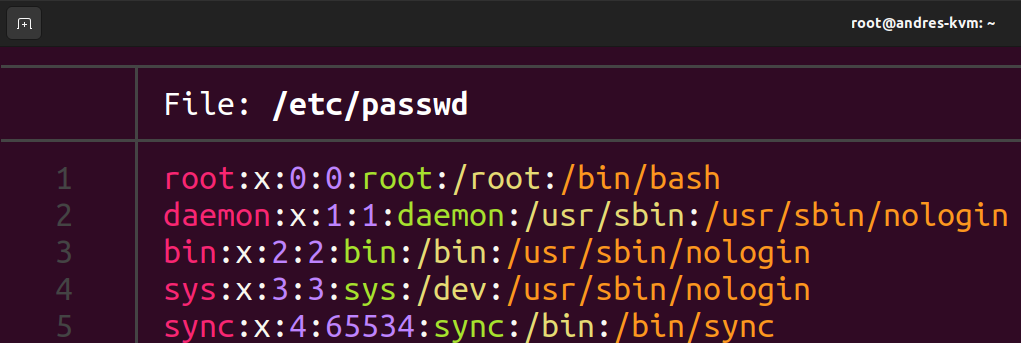
\includegraphics[width=\textwidth]{imagenes/passwdfile.png}
%    \caption{Ejemplo de entradas en el archivo.}
%\end{figure}